\documentclass{standalone}
% main document, called main.tex
\usepackage{amsmath,amssymb}
\usepackage{tikz}
\usetikzlibrary{shapes}
\usepackage{pgfplots}
\usetikzlibrary{calc}
\usetikzlibrary{matrix,arrows,patterns.meta}
\usepackage{graphicx}


%Macros Tikz
\newcommand{\MarqueurH}[3]{\draw[thick,#3] (#1,5pt) -- (#1,-5pt) node[anchor=north] {#2}}
%Marqueur sur l'axe horizontal. Paramètres : Position, nom, couleur
\newcommand{\MarqueurV}[3]{\draw[thick,#3] (5pt,#1) -- (-5pt,#1) node[anchor=east] {#2}}
%Idem sur l'axe vertical


\begin{document}

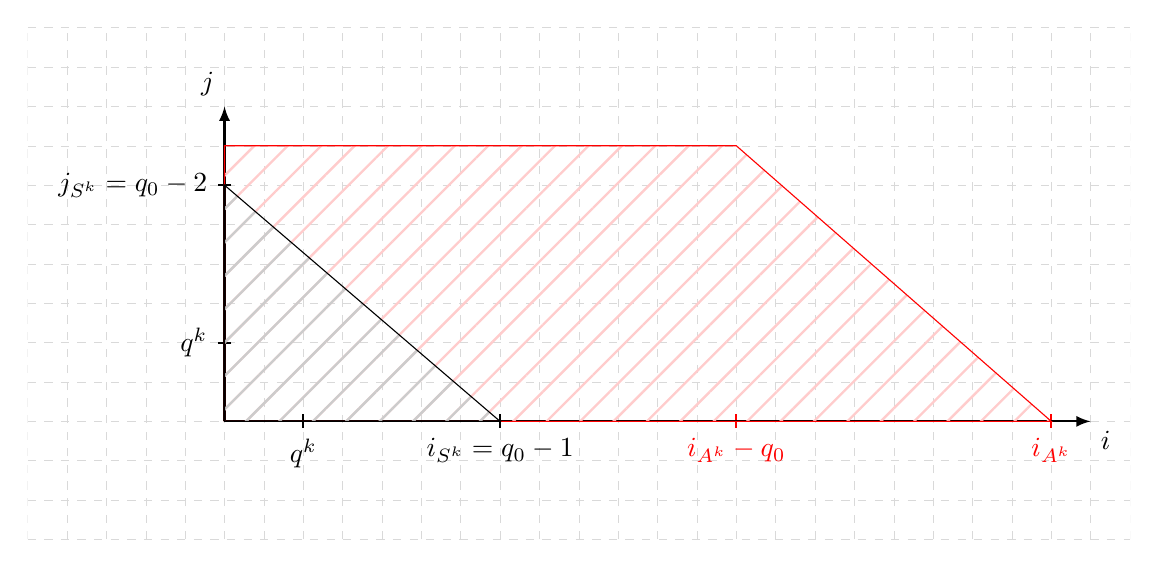
\begin{tikzpicture}[scale=0.5]
	\def\qO{8};
	\def\q{2};
	\def\iAk{21};
	\def\largeur{\iAk+2}
	\def\hauteur{\qO+2}
\clip (-5,-3) rectangle (\largeur,\hauteur); % Clips the picture...
\draw[style=help lines,dashed,opacity=0.3] (-5,-3) grid[step=1cm] (\largeur,\hauteur); % Draws a grid in the new coordinates.

%Sommets des polygones
\coordinate (A) at (\iAk,0) {};
\coordinate (B) at (\iAk-\qO,\qO-1) {};
\coordinate (C) at (0,\qO-1) {};
\coordinate (D) at (0,\qO-2) {};
\coordinate (E) at (\qO-1,0) {} ;

%Marqueurs sur l'axe vertical
\MarqueurV{\q}{$q^k$}{black};
\MarqueurV{\qO-2}{$j_{S^k}=q_0-2$}{black};


%Marqueurs sur l'axe horizontal
\MarqueurH{\iAk-\qO}{$i_{A^k}-q_ 0$}{red};
\MarqueurH{\iAk}{$i_{A^k}$}{red};
\MarqueurH{\q}{$q^k$}{black};
\MarqueurH{\qO-1}{$i_{S^k}=q_0-1$}{black};



%Axes
\draw [thick,-latex] (0,0) -- (0,\qO) node [above left] {$j$};
\draw [thick,-latex] (0,0) -- (\iAk+1,0) node [below right] {$i$};

%Formes
\filldraw [ pattern color=red!20,
	pattern={Lines[
	distance=3mm,
	angle=45,
	line width=0.3mm]},
	draw=red] (0,0) -- (A) -- (B) -- (C) -- cycle;

\filldraw [ pattern color=black!20,
pattern={Lines[
	distance=3mm,
	angle=45,
	line width=0.3mm]},
draw=black] (0,0) -- (E) -- (D)-- cycle;


 
\end{tikzpicture} 




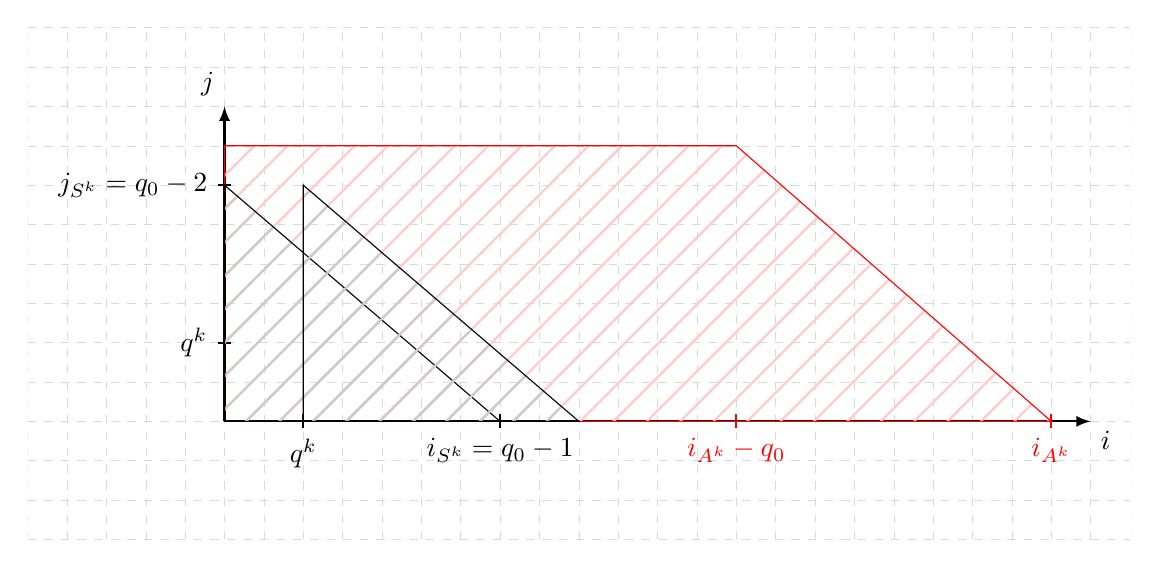
\begin{tikzpicture}[scale=0.5]
	\def\qO{8};
	\def\q{2};
	\def\iAk{21};
	\def\largeur{\iAk+2}
	\def\hauteur{\qO+2}
	\clip (-5,-3) rectangle (\largeur,\hauteur); % Clips the picture...
	\draw[style=help lines,dashed,opacity=0.3] (-5,-3) grid[step=1cm] (\largeur,\hauteur); % Draws a grid in the new coordinates.
	
	%Sommets des polygones
	\coordinate (A) at (\iAk,0) {};
	\coordinate (B) at (\iAk-\qO,\qO-1) {};
	\coordinate (C) at (0,\qO-1) {};
	\coordinate (D) at (0,\qO-2) {};
	\coordinate (E) at (\qO-1,0) {} ;
	
	%Marqueurs sur l'axe vertical
	\MarqueurV{\q}{$q^k$}{black};
	\MarqueurV{\qO-2}{$j_{S^k}=q_0-2$}{black};
	
	
	%Marqueurs sur l'axe horizontal
	\MarqueurH{\iAk-\qO}{$i_{A^k}-q_ 0$}{red};
	\MarqueurH{\iAk}{$i_{A^k}$}{red};
	\MarqueurH{\q}{$q^k$}{black};
	\MarqueurH{\qO-1}{$i_{S^k}=q_0-1$}{black};
	
	
	
	%Axes
	\draw [thick,-latex] (0,0) -- (0,\qO) node [above left] {$j$};
	\draw [thick,-latex] (0,0) -- (\iAk+1,0) node [below right] {$i$};
	
	%Formes
	\filldraw [ pattern color=red!20,
	pattern={Lines[
		distance=3mm,
		angle=45,
		line width=0.3mm]},
	draw=red] (0,0) -- (A) -- (B) -- (C) -- cycle;
	
	\foreach \i in {0,1}{
	\filldraw [ pattern color=black!20,
	pattern={Lines[
		distance=3mm,
		angle=45,
		line width=0.3mm]},
	draw=black] (\i*\q,0) -- ($(E)+(\i*\q,0)$) -- ($(D)+(\i*\q,0)$)-- cycle;
}
	
	
\end{tikzpicture} 

\end{document}